\section{Initial Gene Finding Results} 

In figure~\ref{fig:genecounts}, we see a summary of total genes and mRNAs
predicted by each of the selected tools. An immediate trend can be
seen in this data. The total predicted features for Braker2 are
significantly lower than those from GeneMark in all assemblies except
for \textit{T. reesei}. This may be due to Braker2 using RNAseq data
from \textit{T. reesei} during its training process, which we will
cover in the discussion section. Another observation can be seen when
comparing the predicted genes and predicted RNAs for the same tool
when applied to the assemblies. GeneMark does not appear to identify
any additional isoforms, only reporting the entire gene
structure. Braker2 does identify isoforms, although very few of
them. This may be related to the training set provided to the training
process, although this is not yet confirmed. Overall, it appears that
GeneMark regularly predicts a higher number of features when applied
to these assemblies.

\begin{figure}
  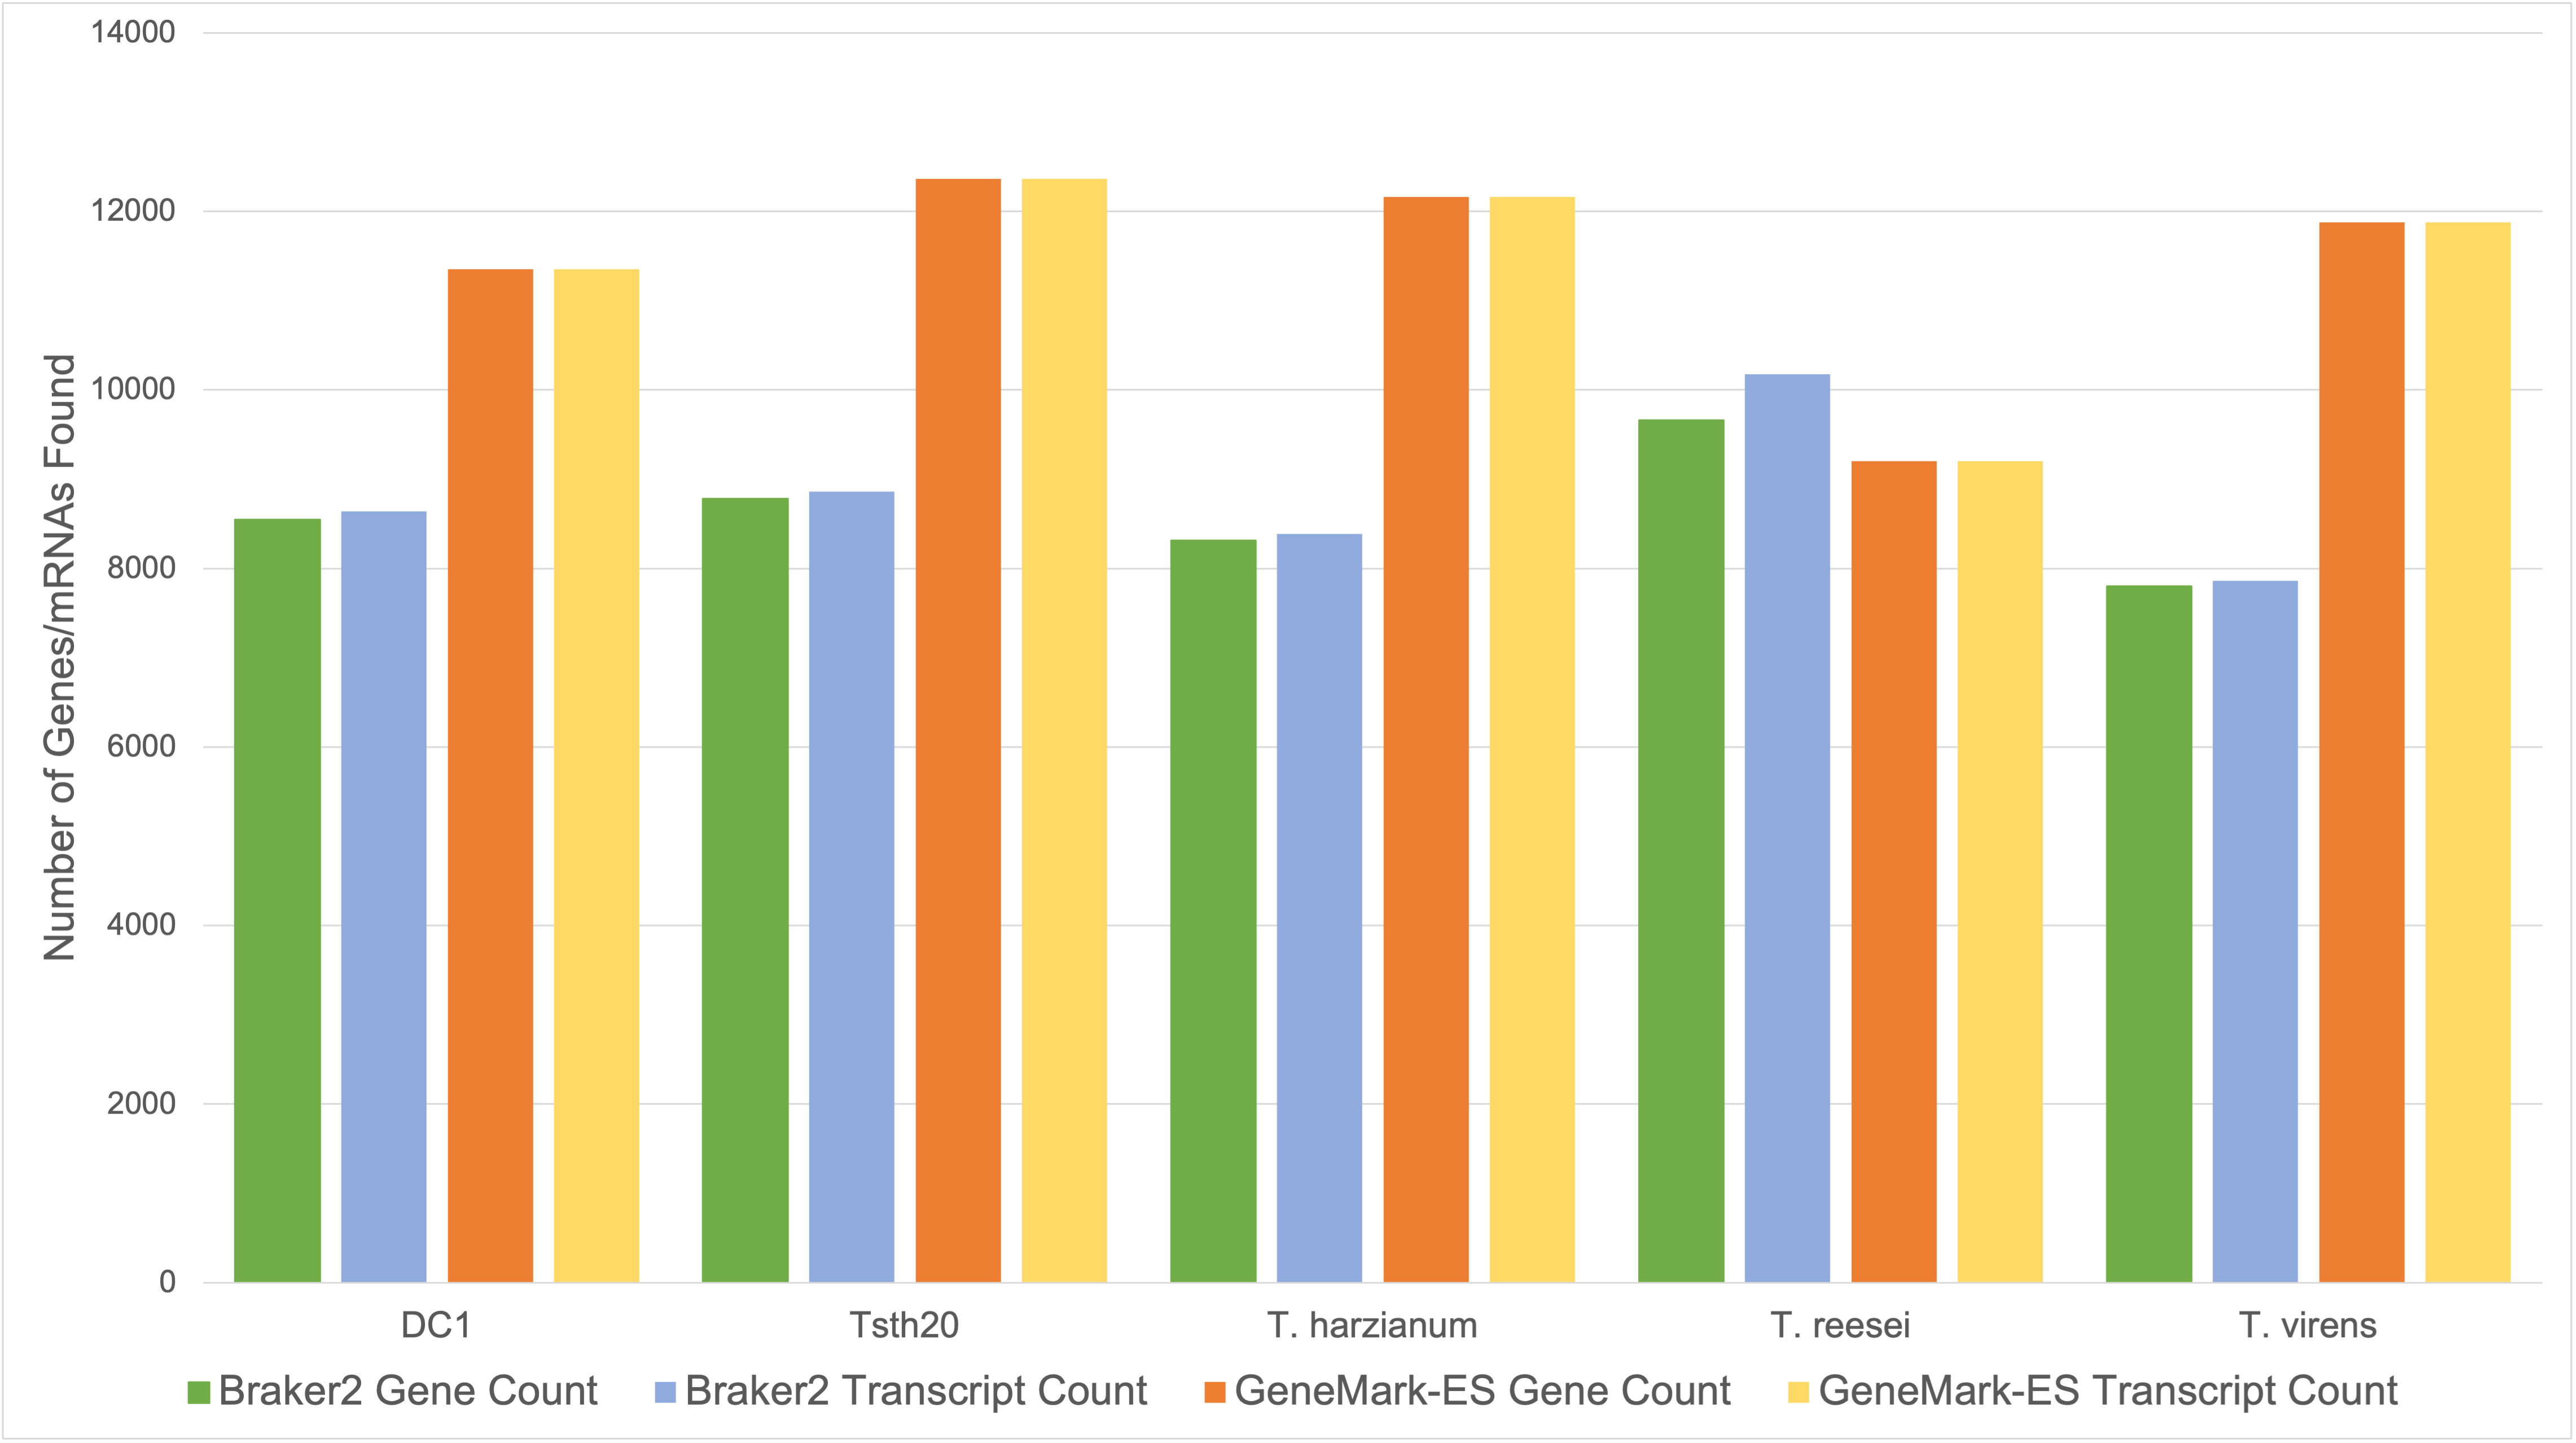
\includegraphics[width=\textwidth]{./figures/nextpolish-gene-finding.png}
  \caption[Counts of predicted genes and mRNAs]{Shows the counts of
    genes and mRNAs found by each gene finding tool for each genome
    assembly considered.}
  \label{fig:genecounts}
\end{figure}

One important ascpect to consider when looking at the output of
different gene prediction tools is the distribution of sequence
lengths predicted by any given tool. Lengths of possible sequences can
vary widely, ranging from small non-coding RNAs, which can be less
than 200 nucleotides in length, up to the largest genes which cover
more than two kilobases. Due to this wide variation in possible
sequence lengths, it is possible that different prediction tools could
produce different distributions of predicted sequence lengths. This is
important if researchers are interested in small non-coding RNAs or
atypically large genes. This section will investigate the coding
sequence lengths predicted by Braker and GeneMark for DC1 and Tsth20
while the RefSeq assemblies will also include the RefSeq annotation.

\section{Distribution of Predicted Gene Lengths}

In, gene finding tools will predict genes of different lengths within
a genome. To better understand the likelihood of a gene being of a
certain length, the cumulative density function for the lengths of CDS
sequences for each gene finding tool are plotted in figure
~\ref{fig:cdf-lengths}. The log base 10 values of gene lengths were
used for a better visulazation of the distributions.In DC1, the curves
from Braker and GeneMark follow each other closely, with the only
variation being genes of short length, where Braker's curve extends
beyond that of GeneMark, indicating that Braker predicts more shorter
genes than GeneMark. In the case of Tsth20, the curves are nearly
identical. In \textit{T. reesei}, we see disagreement in the curves
for shorter genes, with Braker appearing to predict more shorter genes
than GeneMark and RefSeq. The upper portions of the curve trend
towards agreement between the curves. In \textit{T. harzianum}, RefSeq
deviates from GeneMark and Braker, predicting more genes of short
length. Braker and GeneMark appear to be in near-complete
agreement. Finally, in \textit{T. virens}, we see the RefSeq curve
deviating towards more shorted genes once again, although the
deviation is not as drastic as in \textit{T. harzianum}.


\begin{figure}
  \centering
    \begin{subfigure}{0.8\textwidth}
      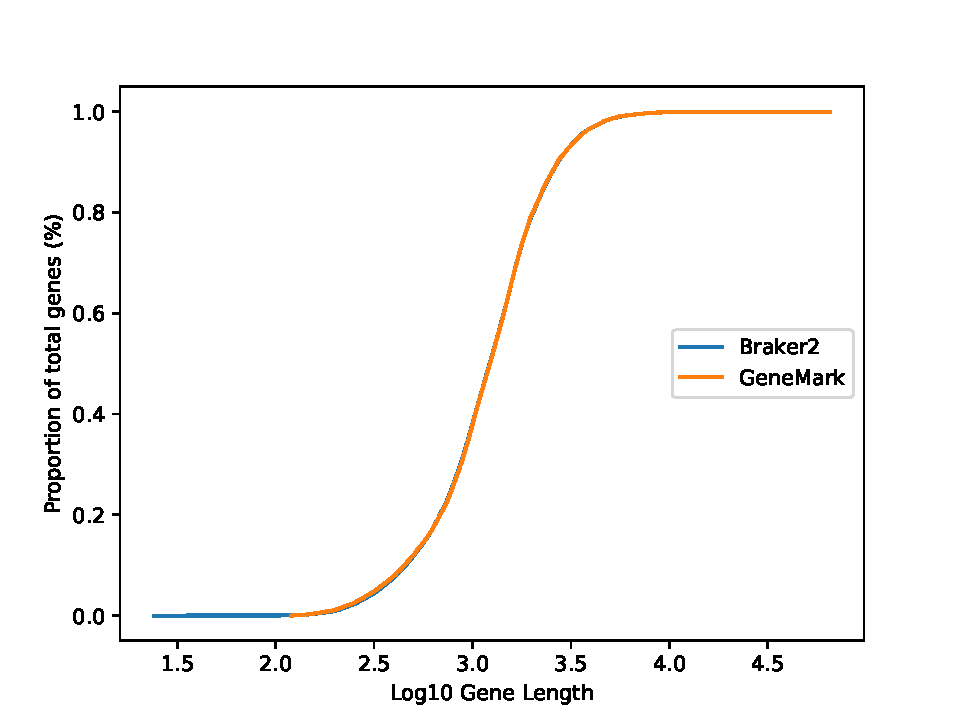
\includegraphics[width=\textwidth]{figures/dc1-cdf-lengths-log.pdf}
      \label{fig:dc1-lengths}
      \caption{DC1}
    \end{subfigure}
    \begin{subfigure}{0.8\textwidth}
      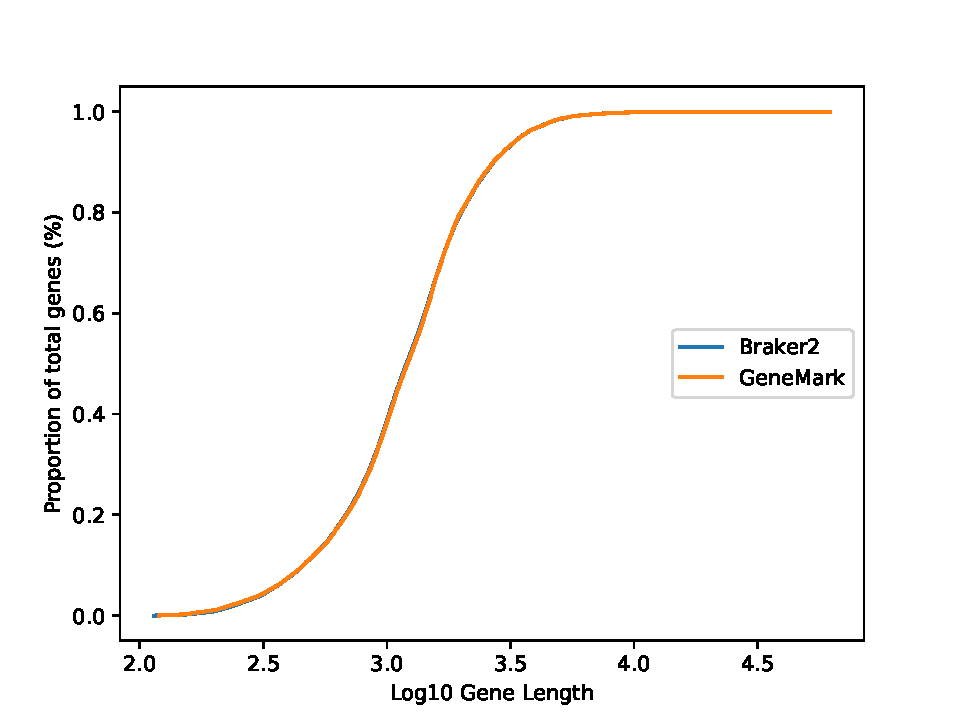
\includegraphics[width=\textwidth]{figures/tsth20-cdf-lengths-log.pdf}
      \label{fig:tsth20-lengths}
      \caption{Tsth20}
    \end{subfigure}
\end{figure}
\begin{figure}[ht]
  \ContinuedFloat
  \centering
    \begin{subfigure}{0.8\textwidth}
      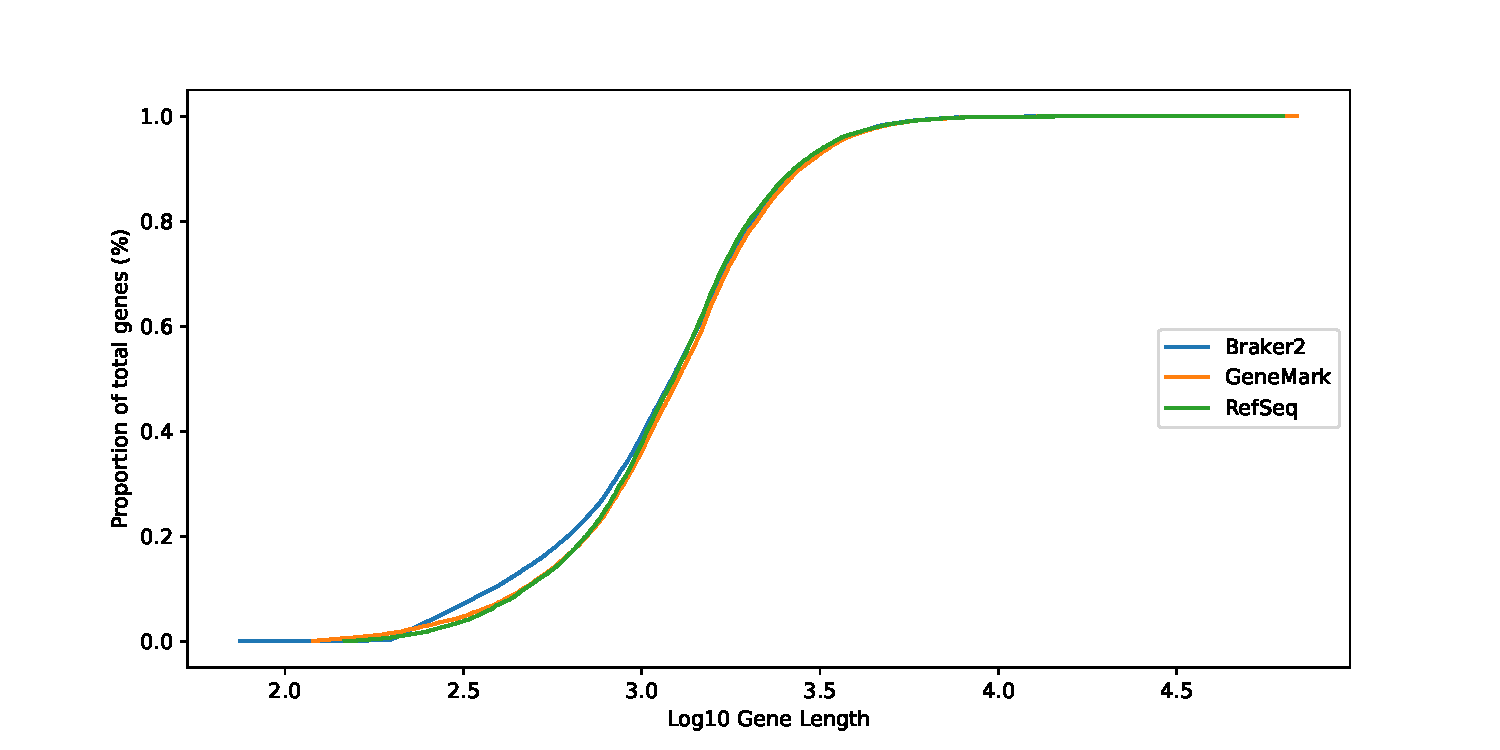
\includegraphics[width=\textwidth]{figures/t-reesei-cdf-lengths-log.pdf}
      \label{fig:treesei-lengths}
      \caption{\textit{T. reesei}}
    \end{subfigure}
    \begin{subfigure}{0.8\textwidth}
      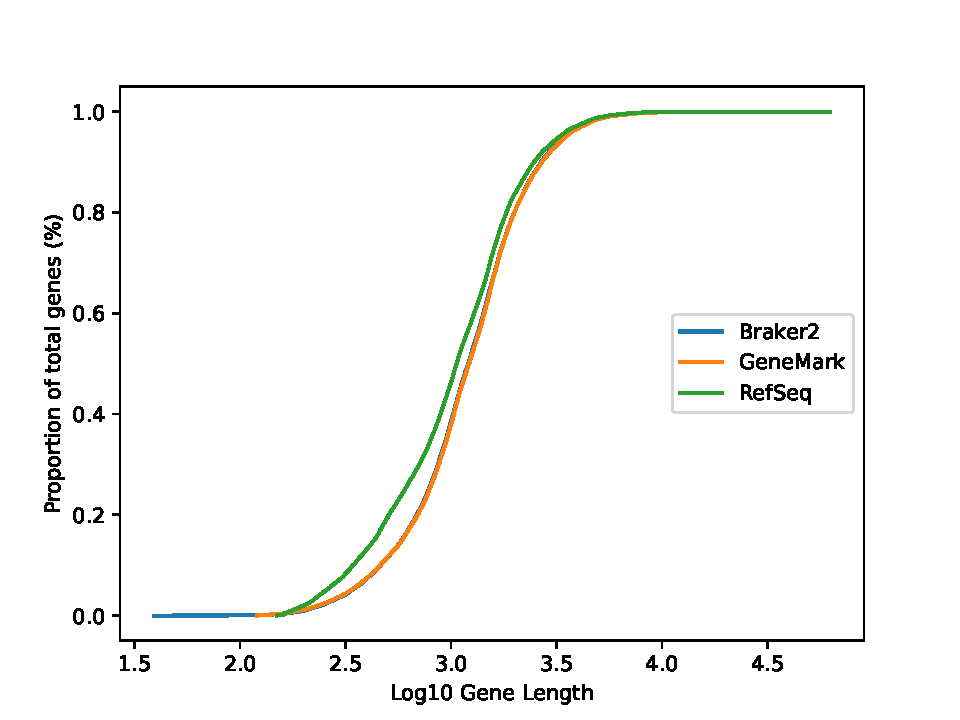
\includegraphics[width=\textwidth]{figures/t-harzianum-cdf-lengths-log.pdf}
      \label{fig:tharzianum-lengths}
      \caption{\textit{T. harzianum}}
    \end{subfigure}
\end{figure}
\begin{figure}[ht]
  \ContinuedFloat
  \centering
    \begin{subfigure}{0.8\textwidth}
      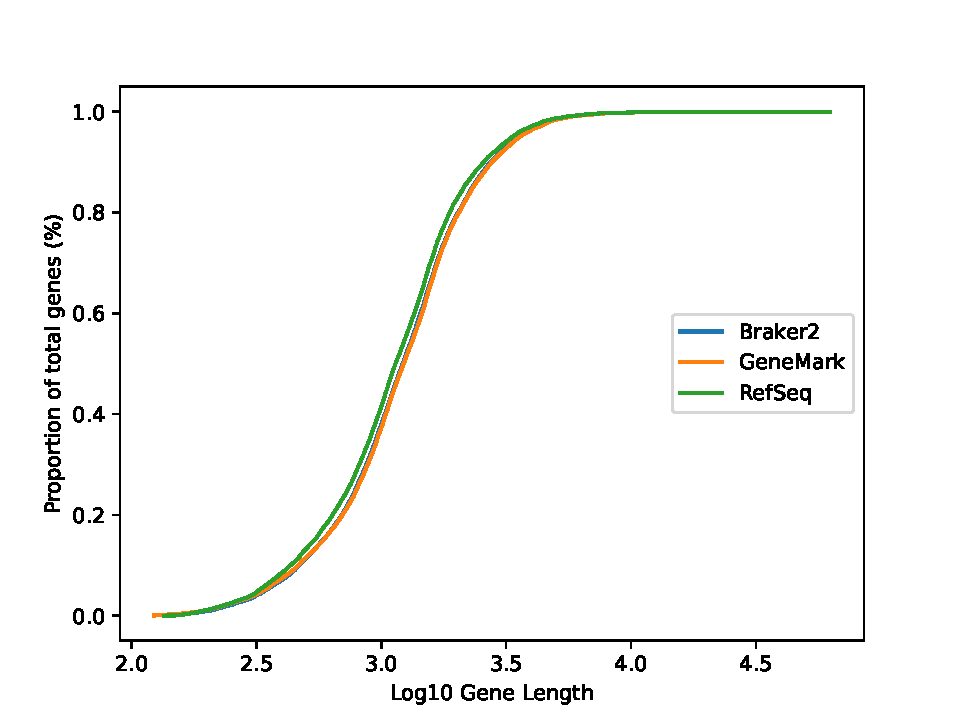
\includegraphics[width=\textwidth]{figures/t-virens-cdf-lengths-log.pdf}
      \label{fig:tvirens-lengths}
      \caption{\textit{T. virens}}
    \end{subfigure}
  \label{fig:cdf-lengths}
  \caption[Cumulative Density Function of Gene Lengths]{Plots of the
    cumulative density function for CDS lengths predicted by each gene
    finding tool.}
\end{figure}

Two-sided two-sample Kolmogorov-Smirnov tests were also performed
using the log10 transformed gene lengths and are presented in table
\ref{table:ks-2s}. In the cases of DC1 and Tsth20, we see that Braker
and GeneMark do not produce statistically different lengths of
genes. In \textit{T. reesei}, while RefSeq and GeneMark do no reject
the null hypothesis when compared, Braker gene lengths are
significantly different than both RefSeq and GeneMark, which is
confirmed visually in the CDF plots above. The same cannot be said for
\textit{T. harzianum}, where RefSeq is significantly different from
both GeneMark and Braker, which are not significantly different from
eachother. This observation extends to \textit{T. virens}.

\begin{table}
  \begin{center}
    \begin{tabular}{|c|c|c|c|c|c|c|}
      \hline
      Genome & Tool \#1 & Tool \#2 & \textit{P}-value  \\ \hline
      DC1 & Braker & GeneMark & $0.999$ \\ \hline
      Tsth20 & Braker & GeneMark & $0.965$ \\ \hline
      \textit{T. reesei} & Braker & GeneMark & $9.481^{-07}$ \\ \hline
      \textit{T. reesei} & GeneMark & RefSeq & $0.002$ \\ \hline
      \textit{T. reesei} & Braker & RefSeq & $1.340^{-07}$ \\ \hline
      \textit{T. harzianum} & Braker & GeneMark & $0.863$ \\ \hline
      \textit{T. harzianum} & GeneMark & RefSeq & $4.313^{-52}$ \\ \hline
      \textit{T. harzianum} & Braker & RefSeq & $4.674^{-55}$ \\ \hline
      \textit{T. virens} & Braker & GeneMark & $0.635$ \\ \hline
      \textit{T. virens} & GeneMark & RefSeq & $7.352^{-12}$ \\ \hline
      \textit{T. virens} & Braker & RefSeq & $1.794^{-09}$ \\ \hline
    \end{tabular}
  \end{center}
  \caption{Table of \textit{P}-values from two-sided two-sample
    Kolmogorov-Smirnov tests between gene finding tools.}
  \label{table:ks-2s}
\end{table}
